\documentclass[11]{article}
\usepackage[margin=1in]{geometry}
\usepackage{amsfonts,amsmath,amssymb}
\usepackage{fancyhdr}
\usepackage{graphicx}
\usepackage{float}
\usepackage{transparent}
\usepackage{eso-pic}
\usepackage[colorlinks,linkcolor={blue}]{hyperref}


\usepackage{listings}
\usepackage{color}


\definecolor{dkgreen}{rgb}{0,0.6,0}
\definecolor{gray}{rgb}{0.5,0.5,0.5}
\definecolor{mauve}{rgb}{0.58,0,0.82}

\lstset{frame=tb,
  language=Java,
  aboveskip=3mm,
  belowskip=3mm,
  showstringspaces=false,
  columns=flexible,
  basicstyle={\small\ttfamily},
  numbers=none,
  numberstyle=\tiny\color{gray},
  keywordstyle=\color{blue},
  commentstyle=\color{dkgreen},
  stringstyle=\color{mauve},
  breaklines=true,
  breakatwhitespace=true,
  tabsize=3
}



\newcommand\BackgroundPic{%
\put(0,0){%
\parbox[b][\paperheight]{\paperwidth}{%
\vfill
\centering
{\transparent{0.3} 
\includegraphics[width=\paperwidth,height=\paperheight,%
keepaspectratio]{background.png}}%
\vfill
}}}

\AddToShipoutPicture*{\BackgroundPic}

\pagestyle{fancy}
\fancyhead{}
\fancyfoot{}
\fancyhead[L]{\slshape \MakeUppercase{Notes}}
\fancyfoot[C]{\thepage}
%\renewcommand{\headrulewidth}{0pt}
\renewcommand{\footrulewidth}{0pt}

\parindent 0ex
\renewcommand{\baselinestretch}{1.5}

\begin{document}
\begin{titlepage}
\begin{center}
\vspace{1cm}
\Large{\textbf{Computer Science 101: Introduction to Java and Algorithms}}\\
\vfill
\line(1,0){400}\\
\huge{\textbf{Section 1: The Fundamentals}}\\
\line(1,0){400}\\
\vfill
Erudition Labs\\
Computer Science 101: Introduction to Java and Algorithms\\
\today\\
\end{center}
\end{titlepage}

\tableofcontents
\thispagestyle{empty}
\clearpage
\setcounter{page}{1}

\section{Terminology}
\begin{itemize}
  \item \textbf{\textit{Source Code}} --
  Use this to refer to the file that has all the code that you the programmer have written. This file is human readable but not machine readable, meaning the computer cannot understand the code in this file. This is the file or files that you give to the compiler to make the machine executable code.

  \item \textbf{\textit{Compiler}} --
	A computer program that we use to translate our source code into machine code that the computer understands.
	
	  \item \textbf{\textit{Syntax}} --
	The grammatical rules of a language.
	
	 \item \textbf{\textit{Declare a variable}} --
	Tell the compiler to set aside memory for a variable, but we do not give the variable a value yet.
	
	  \item \textbf{\textit{Initialize a variable}} --
	We give a variable that we have already declared a value. We can also declare and initialize at the same time.
	
	  \item \textbf{\textit{Library}} --
	Code that somebody else has already written. It was designed for you to use in your code so that you don`t have to re-invent the wheel. There is certain things we we do so often, like output to the standard output, that it was worth the time of creating it so that you don`t have to create it yourself every time you make a program.
	
	\item \textbf{\textit{Concatenation (or concatenate)}} --
	We talk about concatenation when we are putting strings together. We often say things like, ``concatenate A with B``. We just mean that we want to put A and B together as one string.
\end{itemize}

\section{Pre-Chapter}
Pre-Chapters will be optional prerequisites that we think could potentially be useful for the particular Video Series Section (which we use interchangeably with Chapter). Also, throughout these pages, I will talk about origins and things I just find interesting about these topics. If none of this stuff makes sense, don't worry, it`s optional and you can still learn to code and be great at it without this information. Finally, throughout these documents, we will be going over what was covered in the video series as well as go more into depth in some areas and provide additional examples.

\subsection{Binary}
Binary is a mathematical abstraction that we as humans devised in order to encode information discretely and in a boolean logic friendly way. We encode information in sequences of $1$`s and $0$`s. Rather than me explain exactly what binary is, I would recommend that you research it yourself as it`s not really that crucial to beginner programming other than understanding. Perhaps start here \url{<https://www.computerhope.com/jargon/b/binary.htm>}

\subsection{Measuring Storage Space}
As mentioned above, binary is used to encode information into sequences of $1$`s and $0$`s. Since this is a base 2 numbering system, we tend to do things in powers of $2$. If you don't live under a rock, then you have probably heard terms like Gigabyte and Megabyte. But what are these? The smallest unit is called a bit. A bit stores either a $1$ or a $0$. There are 8 bits in a byte. So a byte is used to store sequences of 8 binary bits (8 $1$`s and $0$`s). From here, we use standard SI unit prefixes such as kilo, mega, giga, tera, etc... You can read more about it on wikipedia \url{<https://en.wikipedia.org/wiki/Units_of_information>}\\

\begin{figure}[H]
	\centering
	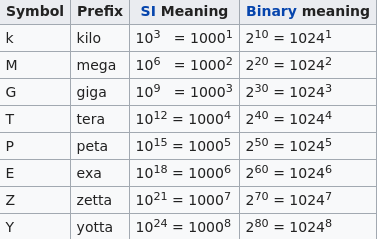
\includegraphics[scale=0.75]{sizes.png}
	\caption{Part of a table taken from \url{<https://en.wikipedia.org/wiki/Units_of_information>}}
\end{figure}

8 bits in a byte, 1024 bytes in a kilobyte, $1024 \times 1024$ bytes in a megabyte, $1024 \times 1024 \times 1024$ bytes in a gigabyte and so on. Why this subsection is useful will make sense once you get to the Types section.

\subsection{What is a Program?}
\paragraph{If you would like to just skip to the more useful stuff about what a program is, look for the next bold face paragraph.}
If you are an absolute beginner to programming or even just the tech world, you may be asking yourself, what is a program and what is programming? To many people computers are a magical black box that just does stuff when they point and click. You, however, have taken the next step by opening up this box to better understand the technology that is commanding our day and age.\\

You see, computers really just reduce down to physics. We can thank the 19th Century Philosopher, Logician and Mathematician, George Boole along with the Potato Famine for all the heavy lifting needed to create the foundations for the Information Age that we currently live in. He invented Boolean Algebra while trying to solve the potato famine and attempt to prove the existence of God. In doing so, he created the mathematics that would become the foundations for digital logic long before we ever had the technology to utilize it.\\

What does any of this have to do with what a program is? Well I just think the inspirational story of George Boole is really underrated and deserves more credit. Anyways, a computer is simply made up of hardware (circuitry) that follows this Boolean Logic. We call the digital logic circuitry, Logic Gates. They perform basic logic operations such as AND, OR and XOR (exclusive OR), etc, much in the same way as you and I do naturally everyday. Although I will not be going into the Logic Gates, we will talk about some of the Logical Operators later. So now we know that a computer is simply a collection of these Logic Gates. My main point here is that computers are not magical, they follow rigorous logic given to us by circuits and thus physics. Everything boils down to an electron moving on a wire.\\

Luckily, you don't really need to know about any of this stuff to start programming. We have had many years to abstract away this complexity to make it easier to use. An interesting question is, how do we go from software to all the electrons moving though wires? Well, we came up with a mathematical abstraction to represent electron flow in wires called binary. The basic idea (and pretty over simplified) is that we use a $1$ to represent giving power to a wire and $0$ to giving no power (aka grounding) a wire. Now we have a way of talking about electric potential. We can string together these $1$`s and $0$`s into sequences and create a special circuit to convert them into electric flow on the wires.\\

What we have done is abstract away the electrical engineering side of computers so that we don't have to worry about it. All we need to do is create the correct sequences of binary numbers to make the computer do stuff. Computers only understand this binary stuff. Well, lets give these special sequences of binary names. Names such as ADD (add two numbers together), MOV (move data around). We often refer to these names as instructions. We can now create a set of instructions so that we don`t have to remember the binary sequences. Instead, we can create a Central Processing Unit (CPU) which has all the circuitry to execute these instructions.\\

Here is an example of an ARM (ARM is a type of instruction set that usually runs things like your phone and small devices) assembly program that I wrote in college:

\begin{figure}[H]
	\centering
	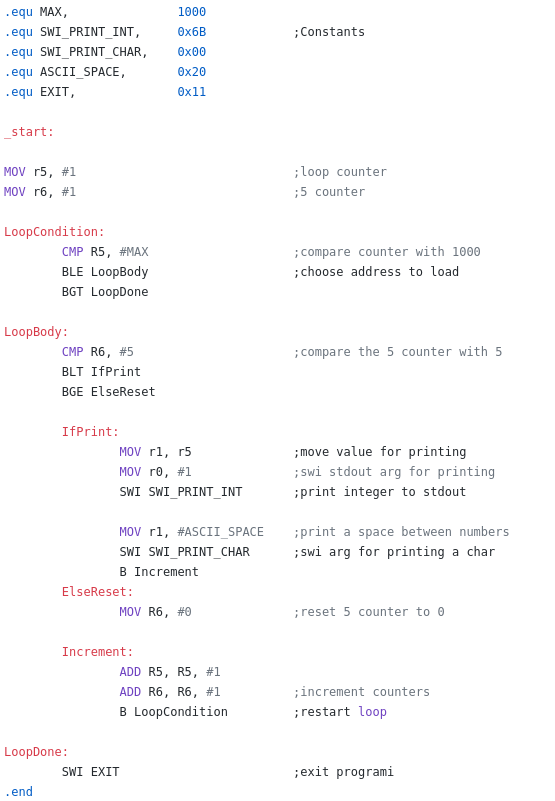
\includegraphics[scale=0.5]{arm.png}
	\caption{ARM assembly program that prints all the integers greater than 0 and less than 1000 that are not divisible by 5}
\end{figure}



Please do not worry about what any of that stuff means. Not even I remember what everything does, and I was the one that wrote it. Yes, people used to write programs like this. In fact, the game Roller Coaster Tycoon was written in assembly. Today, we some people still write small programs like this or they can go into the generated machine instructions and optimize them.\\

Although better, this still looks terrible to remember and write. However, what if we could create a language that is much easier for humans to understand that can be translated into these instructions and thus be run by the computer? In comes high level programming languages such as C, C++ and yes, Java (java is a tad bit different, but the point is the same).\\

\paragraph{HELLO, If you were skipping over all that other stuff that I said you could, now is a good time to start paying attention.} 
According to \href{https://en.wikipedia.org/wiki/Computer_program}{Wikipedia} , "A computer program is a collection of instructions that performs a specific task when executed by a computer." As a programmer, you write these instructions. We use high level programming languages, such as Java, to abstract away the specifics of the internal workings of the computer, to write instructions that both humans and computers can understand. Reread that statement...HUMANS and computers can understand. This is absolutely critical, H-U-M-A-N-S and computers.\\

Now, we start with a plain text file such as the one shown in the video series
\begin{lstlisting}
public class HelloWorld {
    public static void main(String[] args) {
        System.out.println("Hello World!");
    }
}
\end{lstlisting}

This would be saved into a plain text file such has, HelloWorld.java. This file is then compiled. This simply means that we use another program, which we refer to as a compiler, to translate our plain text code into machine instructions. So we are taking the English that is easy for humans to understand and translating it into machine instructions that the machine understands. This new file with the machine instructions is called a program. When you double click that program on your desktop, the machine instructions get loaded into memory and executed one at a time by the Central Processing Unit (CPU). Also a fun fact, your operating system, such as Windows 10, Ubuntu Linux, MacOS, Android, IOS, etc, is a program. So you as a programmer write the program, which gets compiled by another program and loaded/ran using your operating system, which is also a program.\\

\subsection{The Structure of a Java program}
This course will focus on programming using Java. Why use Java? Well, that will be covered in a later section. If we again look at the program from Lecture 1 and 2, 

\begin{lstlisting}
public class HelloWorld {
    public static void main(String[] args) {
        System.out.println("Hello World!");
    }
}
\end{lstlisting}

We can talk about a few things found here. In Java, everything is a class. If you do not know what a class is, don`t worry, we cover that in the upcoming chapters and that phrase will make sense. Java is Object Oriented, again, this will make sense later. The thing I want to talk about here is ``main``. When you write your program, the compiler needs to know where the program starts. Most languages require some entry point into your program so that it knows where to start and most of the time we are required to call it ``main``. Meaning this is the main entry point of the program. Every program you write in Java will have this ``main``. It tells the compiler where to start and then just reads the code from top to bottom, left to right (Just like how you would read anything else in English).

\section{Basic Syntax (Video Series Lecture 1 and 2)}
In this section we will learn about Java keywords, what variables are, what types are and how to print output to your console.
\subsection{Keywords}
If we again look at the code from the video series,
\begin{lstlisting}
public class HelloWorld {
    public static void main(String[] args) {
        System.out.println("Hello World!");
    }
}
\end{lstlisting}
we will see certain things are highlighted colors by the editor. We call this syntax highlighting. It helps us distinguish between different things in our code, such as keywords. Please note that the colors and the syntax highlighting in general all depends on your editor, it has nothing to do with Java. Now from this code snippet, we can see that public, class, static and void are all highlighted blue. The editor does this because it knows that all of these words are Java keywords.\\

A Keyword is a word that is reserved by the programming language. This means that you cannot redefine what the world public, class, void, etc, means. Java has defined what they mean and it is your job to learn what they mean and how to use them. In a sense, the keywords are the Java language. Here is a list of the Java keywords as found in the Java documentation at, \url{<https://docs.oracle.com/javase/tutorial/java/nutsandbolts/_keywords.html>}

\begin{figure}[H]
	\centering
	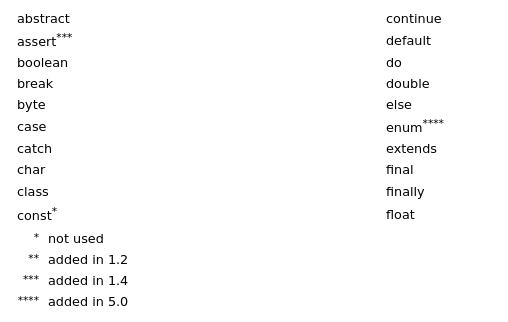
\includegraphics[scale=0.5]{keywords1.png}
	\label{keywords}
\end{figure}

\begin{figure}[H]
	\centering
	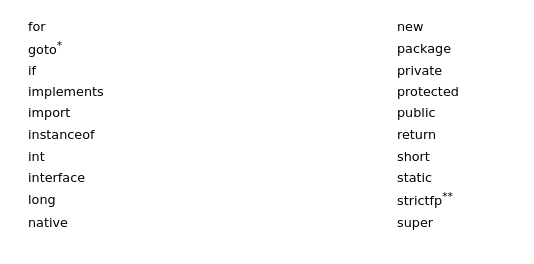
\includegraphics[scale=0.5]{keywords2.png}
\end{figure}

\begin{figure}[H]
	\centering
	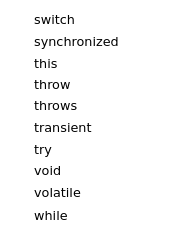
\includegraphics[scale=0.5]{keywords3.png}
\end{figure}

Whenever you write these words in your plain text file, Java will use the definition that they have defined for these words. If you try to redefine them somehow, the compiler will probably give you an error because it simply isn`t allowed.\\


\section{Variables and Types (Video Series Lecture 3 and 4)}
\subsection{Java Types (Primitive Types and Strings)}
Some of these keywords are called data types, particularly, primitive data types. This basically means that these keyword types are used to represent raw data, such as the binary representation of a number. In the video series, we created this table, 
\begin{figure}[H]
	\centering
	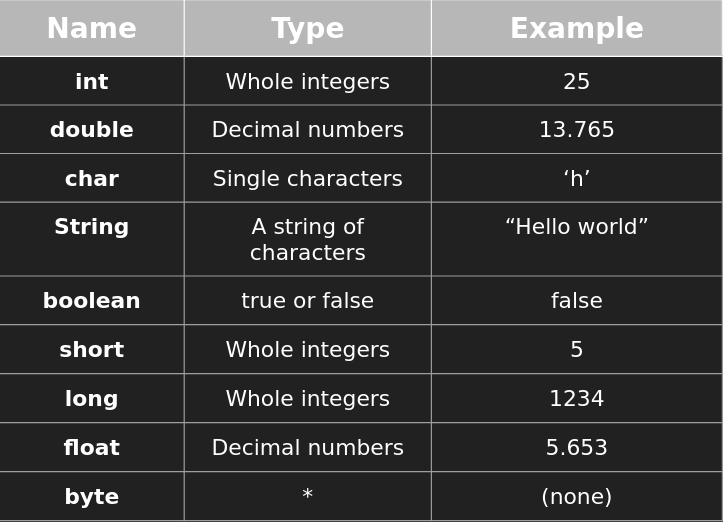
\includegraphics[scale=0.5]{primitives.png}
	\caption{Table from video series lecture 3}
\end{figure}

Notice that all of the names in the table are in the reserved keywords list from \ref{keywords}, except ``String``. We include the String in the table because it is extremely common to use, however, it is not a primitive data type, it is an object. For now, there is no need to worry about what the difference actually is.\\

Take a look at the above table and notice that  int, short and long all store whole integers. Similarly, float and double both store decimal values. So why have these keywords that all do the same thing? The answer is, they store different sizes. Sizes of what? Let`s take an example. Int stores the binary representation of the whole integer. So to store larger numbers, we need more bits (more $1$`s and $0$`s) to uniquely represent that number. And thus we need more storage space to store those extra bits. Take a look at the following table and notice which types have more storage space and thus can store a larger range of values.

\begin{center}
  \begin{tabular}{ | c | c | c | }
    \hline
    Type & Size & Range \\ \hline
    boolean & 1 bit & true or false \\ \hline
    byte & 8 bits (1 byte) & [-128, 128] \\  \hline
    short & 16 bits (2 bytes) & [-32768, 32767] \\ \hline
    char & 16 bits (2 bytes) & [0, 65535] \\ \hline
    int & 32 bits (4 bytes) & [-2147483648, 2147483648] \\ \hline
    long & 64 bits (8 bytes) & [$-2^{63}$, $2^{63}$ -1] \\ \hline
    float & 32 bits (4 bytes) & 32-bit IEEE 754 floating-point \\ \hline
    double & 64 bits (8 bytes) & 64-bit IEEE 754 floating-point\\
    \hline
  \end{tabular}
\end{center}

Notice that long has a much larger range for the values it can handle in comparison to int due to the extra space that the keyword type allows. When your code is compiled, these types tell the compiler how much space to set aside for the value it is going to store. But what happens if we go over the range? This is called overflow. For example, in the case of int, if we stored larger that $2,147,483647$, we would have integer wrap (aka integer overflow). This means that we have run out of unique ways of representing integers so we lose some of the bits. The resulting bits that get stored just so happens to be the same as some other number in that range. So if we go slightly over the max number in the int range, what gets stored is probably some negative number on the other end of the int range. \\

A classic example of integer wrap is the Y2K bug. You can read about it \url{https://searchwindowsserver.techtarget.com/definition/Y2K-year-2000} But essentially we were storing years as two digits $00$ to $99$. So the year $1995$ would be stored as $95$ and the year $1900$ would be stored as $00$. This was done because back in those days, we had to be extremely conservative with memory storage space. Well in the year $2000$ (just like when we reach the end of the int range) we ran out of unique ways to store years. So the year $2000$ would be stored as $00$ which is actually the opposite end of the range, namely year $1900$. The year wrapped around to the beginning of the range. So we thought the world was going to burn, planes would crash, the stock market would crash, aliens would invade, and cows would be abducted. But nothing really happened. It is however an example of overflow, aka integer wrap in this case. \\

In case you were wondering what this IEEE 754 floating-point thing is. IEEE is  a group that sets standards for companies who make computers. This way, computers can be universal and interact with each other despite having different hardware and software designs. One such standard is the way we store decimals in binary. You can read about it \url{<https://en.wikipedia.org/wiki/IEEE_754>} also if you would like to read more about primitive data types, check out the javadocs tutorials found at \url{<https://docs.oracle.com/javase/tutorial/java/nutsandbolts/datatypes.html>} \\

\subsection{Variables}
Variables are ways that you can store things under a name. From the video series, we show that variables take the form of
\begin{center}
  \begin{tabular}{ | c | c | c | c |}
    \hline
    TYPE & $VARIABLE\_NAME$ & $=$ & VALUE  \\
    \hline
  \end{tabular}
\end{center}

Variables are often used to store values that you do not know until the program is running. Often times we need to pass around a value that is often changing. In the video series, we showed basic usage of declaring variables with a value.

\begin{lstlisting}
public class HelloWorld {
    public static void main(String[] args) {
        int number = 5;
        double score = 97.3;
        char letter = 'h';
        String hello = "Hello World!";
        bool understands = true;
    }
}
\end{lstlisting}

We can also do things like copy values from one variable into another or reuse variables that are already declared.

\begin{lstlisting}
public class HelloWorld {
    public static void main(String[] args) {
        int number = 5;
        double score = 97.3;
        char letter = 'h';
        String hello = "Hello World!";
        bool understands = true;
        
        int newNumber = number;
        number = 0;
        understands = false
    }
}
\end{lstlisting}
 In this case, newNumber will equal $5$ and then on the next line, number will equal $0$ but newNumber will still equal $5$ since it made its own copy before number was reassigned.

\section{Math in Code (Video Series Lecture 5)}
Java provides basic arithmetic operators for you to use, namely division, multiplication, subtraction and addition. We created this simple table in the video series.
\begin{figure}[H]
	\centering
	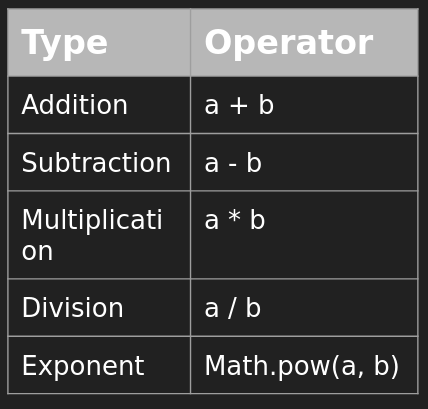
\includegraphics[scale=0.5]{math1.png}
	\caption{Table from video series lecture 5}
\end{figure}

The table is pretty self explanatory, but why did we include Math.pow(a,b) ? Well for most things other than the basic math operation, you will need to use some external library such as Java's Math library. If you are unsure what a library is, don't worry about it too much yet, but a library is basically code that someone else has written for you to use. The math section is pretty straight forward. Java follows basic math precedence. That is to say that multiplication and division will be done before addition and subtraction unless you specify otherwise. If you want to set the order of precedence yourself, you can wrap things that you want done first in parenthesis, just like normal math.\\

For example, $5 + 2 * 3$ will be evaluated as $5 + (2 * 3)$ \\
However, if you want the addition done first, you can write it as $(5 + 2) * 3$\\
\pagebreak
\begin{lstlisting}
public class HelloWorld {
    public static void main(String[] args) {
        int number = 3;
        System.out.println(number + 17);

        System.out.println(number);
        number = number + 7;
        System.out.println(number);
    }
}

\end{lstlisting}

If you recall this code snippet from the video series, you will see that you can use variables with the arithmetic operators as well. I will now show another code snippet with more examples and with precedence.

\begin{lstlisting}
public class HelloWorld {
    public static void main(String[] args) {
        int number = 3;
        System.out.println(number + 17);

        System.out.println(number);
        number = number + 7;
        System.out.println(number);
        
        int anotherNumber = 5 + number;
        
        int sum = anotherNumber + number;
        int sumWithPrecedence = (anotherNumber * sum) + ( number - 5)
    }
}

\end{lstlisting}
As you can see, if you are familiar with basic arithmetic, then you can also do it in code.

\subsubsection{A Note about $\%$}
This may be a little advanced unless you have taken a Discrete Mathematical Structures class or studied number theory on your own. For most people, knowing that the modulus operator will give you the remainder of integer division is enough. So feel free to skip this. For those that want to know more, read on.\\

The modulus operator comes from number theory when we are talking about equivalence relations and congruences. The technical definition of $\%$ (math use (mod) so I will be switching to the mathematical notation) is:\\
$x$ $\equiv$ $y$ ($mod$ $m$) is true if $x$ $mod$ $m$ $=$ $y$ $mod$ $m$\\
that is to say\\
$x$ $\equiv$ $y$ ($mod$ $m$) if $m$ $|$ $x$ $-$ $y$\\

in some more English that says $x$ is equivalent to $y$ ($mod$ $m$) if $m$ divides $x$ - $y$\\
To better illustrate what modulus division does when programming, let us take an example. Let`s say we want the remainder of $16$ $\div$ $6$. In another form we want to know why \\
$16$ $\%$ $6$ $=$ $4$\\
First it performs $integer$ $division$, (this means that any fractional number is dropped which is equivalent to rounding down)\\
So, $16$ $/$ $6$ $=$ $2$\\
Then multiple the result with the divisor\\
$2$ $*$ $6$ $=$ $12$\\
Now subtract the result from the above multiplication with the dividend\\
$16$ $-$ $12$ $=$ $4$\\

Why does the distinction between modular arithmetic and just getting the remainder matter? Well because modular arithmetic asserts, for example that $23$ and $1903$ are equivalent $mod$ $10$. What does this mean? (For programming, nothing really, but basically it means they have the same remainder when you divide by $10$), however it`s beyond the scope of this lecture series. If you would like to learn more, check out number theory. Perhaps a good place to look at is \url{<http://www.cs.ecu.edu/karl/6420/spr16/Notes/Tool/numbers.html>}
\end{document}